\chapter{Design}

For bedre at forstå designet omkring spillet, har vi ud fra use case 1 (Tabel \ref{usecase:1}), lavet et klassediagram som beskriver de elementer spillet består af.
Det ses der, at spillet kommer til at bestå af terningerne og spillere.
På figur \ref{fig:klassediagram} ses klassediagrammet.

\section{Klassediagram}

\begin{figure}[h]
    \begin{center}
        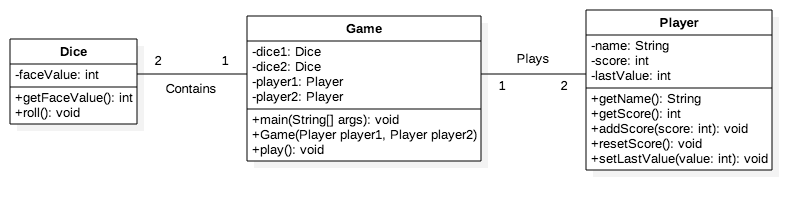
\includegraphics[width=15cm]{graphics/Klassediagram}
        \caption{Klassediagram over spillet}
        \label{fig:klassediagram}
    \end{center}
\end{figure}

\section{Flowdiagram}
\begin{tikzpicture}[node distance=2cm]
\node (start) [startstop] {Spillet startes};
\node (kast) [process, below of=start] {Terningerne kastes};
\node (sum) [process, below of=kast] {Summen bestemmer felt};
\node (felt) [process, below of=sum] {Feltet giver point};
\node (hvis) [decision, below of=felt, yshift=-1.5cm] {Pointsum $\geq$ 3000?};
\node (nyspiller) [process, left of=felt, xshift=-4cm] {Næste spillers tur};
\node (vinder) [startstop, below of=hvis, yshift=-1.5cm] {Spillet afsluttes};
\draw [arrow] (start) -- (kast);
\draw [arrow] (kast) -- (sum);
\draw [arrow] (sum) -- (felt);
\draw [arrow] (felt) -- (hvis);
\draw [arrow] (hvis) -- node[anchor=east] {Ja} (vinder);
\draw [arrow] (hvis) -| node[anchor=north] {Nej}  (nyspiller);
\draw [arrow] (nyspiller) |- (kast);
\end{tikzpicture} 
